\chapter{Tutorial}

\section{Getting started}

\subsection{Kobold Server}
There are two ways to start and use the Kobold Server - {\it stand-alone} or from
{Eclipse}. In both cases make sure, that you edit the server.properties
file from {\it kobold.server/server.properties} to suite your local
requirements. Under UNIX this file might look similiar to the following
bits:

\begin{verbatim}
# Note storePath is the prefix path for all kobold stores!
kobold.server.storePath=/tmp/
kobold.server.globalMessageStore=global.xml
kobold.server.messageStore=messages.xml
kobold.server.productStore=product.xml
kobold.server.userStore=user.xml
#
java.protocol.handler.pkgs=com.sun.net.ssl.internal.www.protocol
javax.net.debug=all
javax.net.ssl.keyStore=../kobold.common/scripts/keystore
javax.net.ssl.keyStorePassword=kobold1
javax.net.ssl.trustStore=../kobold.common/scripts/truststore
javax.net.ssl.trustStorePassword=kobold1
\end{verbatim}

Under Windows-based systems you've to change the paths into a
DOS-alike format.

In the following table all properties are described in detail:

\begin{tabular}{|l|l|l|}\hline
\textbf{Property} &  \textbf{Description}\\ \hline
kobold.server.storePath  & destination path for files stored by the server \\ \hline
kobold.server.globalMessageStore & file name to store global messages \\
    \hline
kobold.server.messageStore & file name to store pending messages \\
    \hline
kobold.server.productStore & file name to store products and
productlines \\ \hline
kobold.server.userStore & file name to store user data \\ \hline
java.protocol.handler.pkgs & default protocol to commincate \\ \hline
javax.net.debug & debug level of net communication \\ \hline
javax.net.ssl.keyStore & path to your SSL keystore \\ \hline
javax.net.ssl.keyStorePassword & password to access your SSL keystore \\
    \hline
javax.net.ssl.trustStore & path to your SSL truststore \\ \hline
javax.net.ssl.trustStorePassword & password to access your SSL
truststore \\ \hline
\end{tabular}

To start the Kobold server within Eclipse just select 'Run...' in the
'Run' menu from
Eclipse and select the class
{\it kobold.server.SecureKoboldWebServer} with a numerical argument for
the port it should listen for connections. The working directory must be
the directory where your {\it server.properties} are located.

To start the Kobold server from the console just enter following
command within the directory where your {\it server.properties} file is
located:

\begin{verbatim}
java kobold.server.SecureKoboldWebServer 23232
\end{verbatim}

Make sure that your {\it \$CLASSPATH} environment contains all JARs
provided by {\it kobold.common/contrib} beside a Java2 JRE and the Sun
JSSE classes (included by Sun JDK 1.4).

\subsection{Kobold Client Feature Set}
Similiar to the Kobold server, the kobold client feature set contains
a file {\it client.properties} located in {\it
kobold.client.plam/client.properties} which has to be edited to
suite your local requirements.

\begin{verbatim}
# Used for SSL based communication
java.protocol.handler.pkgs=com.sun.net.ssl.internal.www.protocol
javax.net.debug=all
javax.net.ssl.keyStore=/home/garbeam/eclipse/kobold.common/scripts/keystore
javax.net.ssl.keyStorePassword=kobold1
javax.net.ssl.trustStore=/home/garbeam/eclipse/kobold.common/scripts/truststore
javax.net.ssl.trustStorePassword=kobold1
\end{verbatim}

As you can see, it contains the same properties as the {\it
server.properties} file for SSL communication, but since the Kobold
client is independent from the server it has it's own properties.

To start the Kobold client feature set from within Eclipse (which is
currently the only way) just select 'Run...' in the 'Run' menu and
double-click 'Run-time Workbench'. A new configuration is created which you 
can name as you wish (see \ref{run}). 

\begin{figure}[h!]
\begin{center}
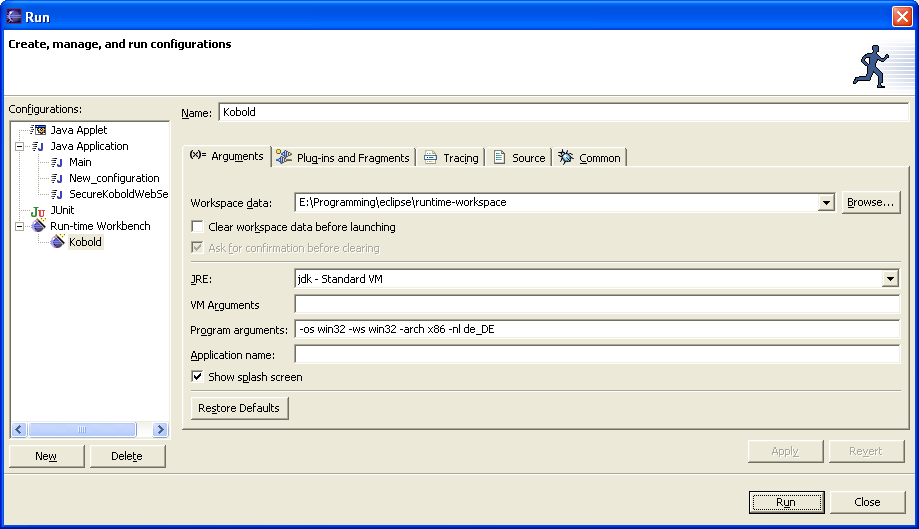
\includegraphics[width=15cm]{run.png}
   \caption{This is how your buildpath should look like}
\label{run}
\end{center}
\end{figure}\par

You've to enter only one VM argument which is needed to locate the {\it
client.properties} file and to suite your local requirements: \par

\begin{verbatim}
-Dkobold.client.configFile=/home/garbeam/eclipse/kobold.client.plam/client.properties
\end{verbatim}

Confirm with 'Run'.

A new Eclipse instance will open with the Kobold feature set enabled.

\section{Checking out a product(line)}

In the File menu select 'New' and then 'Kobold PLAM Project'. The Kobold wizard opens.
Enter the name of the project you want to create (see \ref{wizard1}).

\begin{figure}[h!]
\begin{center}
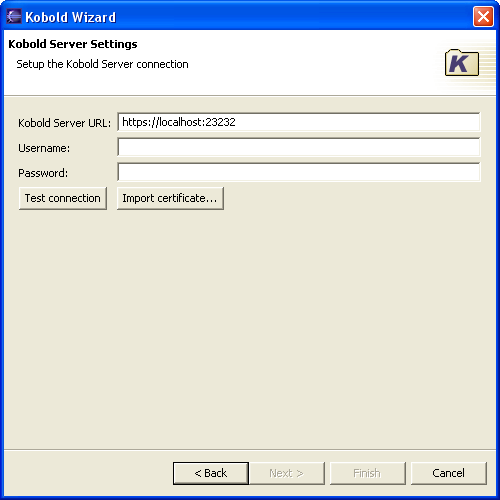
\includegraphics[width=10cm]{wizard1.png}
   \caption{Kobold wizard}
\label{wizard1}
\end{center}
\end{figure}\par

After that enter the url of your Kobold server, your username and password (see \ref{wizard2}).

\begin{figure}[h!]
\begin{center}

\includegraphics[width=10cm]{wizard2.png}
   \caption{Kobold wizard}
\label{wizard2}
\end{center}
\end{figure}\par

In the last step you have to choose the productline (see \ref{wizard3}).

\begin{figure}[h!]
\begin{center}
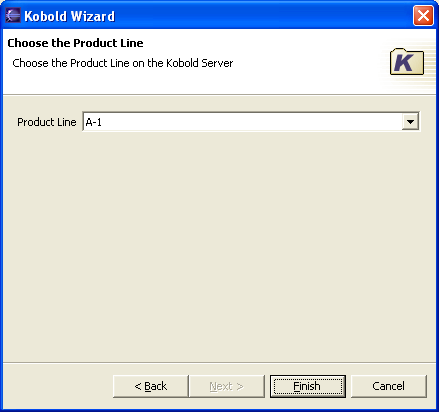
\includegraphics[width=10cm]{wizard3.png}
   \caption{Kobold wizard}
\label{wizard3}
\end{center}
\end{figure}\par

A new project has been created. You can open the different views through the Window menu
and 'show view'. 
